%!TEX root = paper.tex

We propose \emph{latent ranker algorithm (LRA)} for solving the personalized ranking problem. The pseudocode of the algorithm is in \cref{alg:latent-rank}. LRA has two components, column learning and row ranking. The column learning algorithm recommends a list of $d$ columns. The row ranking algorithm recommends an ordering of these columns. The column learning algorithm is the same as in  \citet{radlinski2008learning}. But we exploit the additional structure in our problem to show a stronger regret bound. It consists of $d$ instances of multi-armed bandit (MAB) algorithms, which we denote by $\textrm{MAB}_k(n)$ for $k \in [d]$. $\textrm{MAB}_1(n)$ learns the most rewarding column on average, $\textrm{MAB}_2(n)$ learns the most rewarding column on average conditioned on the first learned columns, as so on. The row learning algorithm are multiple instances of the weighted majority algorithm, for each user. More precisely, for each user $i$ and each set of $d$ columns $J$, we have an instance of the weighted majority algorithm $\textrm{WMA}_{i, J}(n)$ with $d!$ arms, which correspond to all possible permutations of $J$. The objective of $\textrm{WMA}_{i, J}(n)$ is to learn a permutation of $J$ with the highest reward, as measured by \eqref{eq:reward}.

LRA interacts with the environment as follows. At time $t$, a uniformly random user $i_t$ is revealed to LRA. Then, in the ascending order of $k \in [d]$, $\textrm{MAB}_k(n)$ suggests a column $\ell_{t, k}$. If $\textrm{MAB}_{k + 1}(n)$ suggests a previously suggested column in $\{\ell_{t, 1}, \dots, \ell_{t, k}\}$, then $\ell_{t, k + 1}$ is chosen uniformly at random from the remaining columns. We denote the set of $d$ selected columns by $J_t = \{\ell_{t, 1}, \dots, \ell_{t, d}\}$. Then, the weighted majority instance $\textrm{WMA}_{i_t, J_t}(n)$, for user $i_t$ and columns $J_t$, selects a permutation $\pi_{t, i_t}$ of $J_t$.

The user is recommended the permuted list of items, $\pi_{t, i_t}(J_t)$, and LRA observes the individual rewards of all recommended items. After this, we update both column and row learning algorithms. The reward of $\textrm{MAB}_k(n)$, which selects the $k$-th column in $J_t$, is $\max_{j \in [k]} r_t(i_t, \ell_{t, j}) - \max_{j \in [k - 1]} r_t(i_t, \ell_{t, j})$. That is, the reward is the marginal gain of that column over previously chosen columns. Since LRA observes the individual rewards of all recommended items, we can compute the reward of any permutation of $J_t$ in row $i_t$. These rewards are then used to update $\textrm{WMA}_{i_t, J_t}(n)$. An illustrative diagram of the entire learning process is shown in \cref{fig:rankedbandit}.

\begin{figure}
    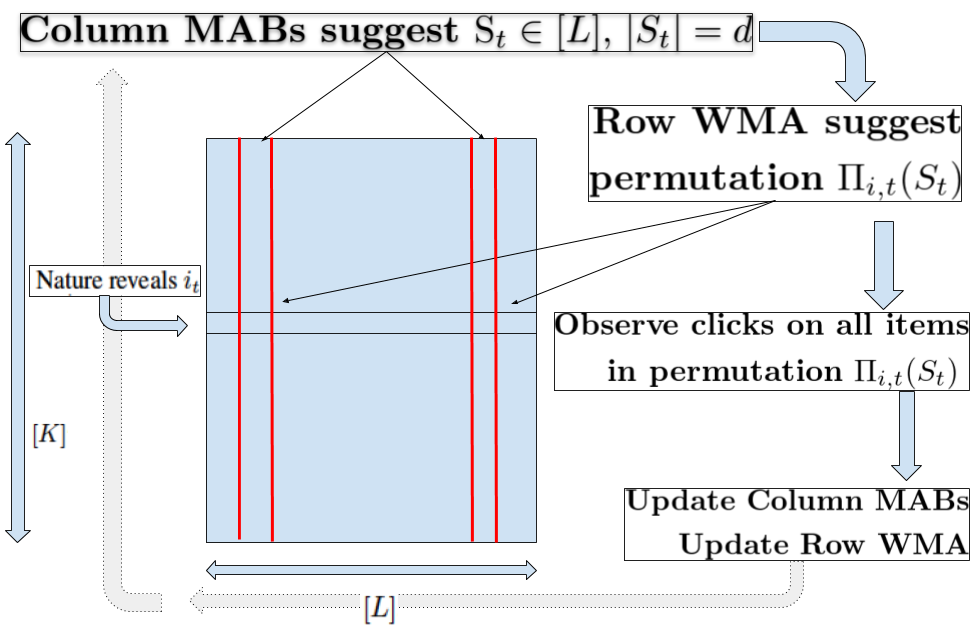
\includegraphics[scale=0.2]{img/RankedBand.png}
    \caption{Latent Ranked Bandit in rank $d=2$ scenario. \todob{The figure is super confusing. If you want to have it, add a flow chart.}}
    \label{fig:rankedbandit}
    \vspace*{-1em}
\end{figure}

\begin{algorithm}
\caption{Latent Ranker Algorithm}
\label{alg:latent-rank}
  \begin{algorithmic}[1]
  \State \textbf{Input:} Rank $d$, horizon $n$.
  \State Initialize MAB$_k(n)$ for $i=1,...,d$
  \State Initialize WMA$_{i,J}(n)$ for $i \in [K], J \subset [L], |J| = d.$
    \For{$t = 1, \dots, n$}
      \State User $i_t$ comes to the system
      \For{$k = 1, \dots, d$}
      %\State // Choose $d$ items from $d$ column MABs
      \State $\hat{{\ell}}_{k,t} \leftarrow$ suggest item $MAB_k(n)$
      \If{$\hat{{\ell}}_{k,t} \in \{ \ell_{1, t},\dots,\ell_{k-1, t}\}$}
      \State ${\ell}_{k,t} \leftarrow$ select arbitrarirly from the remaining
      \Else
      \State $\ell_{k,t} \leftarrow \hat{\ell}_{k,t}$
      \EndIf
      \EndFor
      \State $(\tilde{\ell}_{1,t},\tilde{\ell}_{2,t},\dots,\tilde{\ell}_{d,t} )\leftarrow$ WMA$_{i_t,\{ l_{1,t},...,l_{d,t} \} }$ %by sampling  according to $p_{i_t,1},p_{i_t,2},\dots,p_{i_t,d!}$.
      %by sorting descendingly according to $w_{i_t,1},w_{i_t,2},\dots,w_{i_t,d}$.
      \State Let  $\{ r_{t}(\ell_{1,t}), r_{t}(\ell_{2,t}),\dots,r_{t}(\ell_{d,t}) \}$ be the user feedback.
      \State Let $f_t(\ell_{i,t}) = \max \{ r_t(\ell_{1,t}),...,r_t(\ell_{i-1,t}),r_t({\ell}_{i,t}) \} - \max \{ r_t(\ell_{1,t}),...,r_t(\ell_{i-1,t}) \}$ 
      \State update(MAB$_{k}(n)$, reward = $f_t(\ell_{k,t})$, arm = $\hat{\ell}_{k,t}$)
      \State update(WMA$_{i_t,J_t}$,$\{ r_t(\ell_{1,t}),...,r_t(\ell_{d,t})\}$ )
    \EndFor
%    \Procedure{UpdateColumnMAB}{}
%    \For{$k = 1, \dots, d$}
%    \State Update MAB$_k(n)$ with feedback $f_{k,t} = \max_{j\in [k]} r_t(i_t, \ell_{j,t}) - \max_{j\in [k-1]} r_t(i_t,\ell_{j,t})$
%    % where $J_t[1: k] = \lbrace r_{t}({\ell}_{1,t}), r_{t}({\ell}_{2,t}),\dots,r_{t}({\ell}_{k,t})\rbrace$
%    \EndFor
%\EndProcedure
%\Procedure{UpdateRowWMA}{$i_t$}
%	\For{$k=1,2,\dots,d!$}
%	\State $r_k = 0$ \Comment{Calculate weighted sum of rewards}
%    \For{$j = 1, \dots, d$}
%    \State $r_{k} = r_{k} + \frac{1}{j}r_{t}(\tilde{\ell}_{j,t})$
%    \EndFor
%    \State $w_{i_t,k} = w_{i_t,k} + r_k$  \Comment{Update weights}
%    \EndFor
%	\For{$k = 1, \dots, d!$}
%	\State $p_{i_t,k} = \dfrac{\exp(w_{i_t,k})}{\sum_{b=1}^{d!} \exp(w_{i_t,b})} $ %\Comment{Update probabilities}
%	\EndFor
%\EndProcedure
  \end{algorithmic}
\end{algorithm}

\todoan{Probably need to add a bit more explanation about the rewards of MABs}
